\begin{figure}[htbp]
\centering
% Encoder colors (reuse from Nature CNN)
\definecolor{encfade}{HTML}{B8D2E6}
% SPR-specific component color
\definecolor{sprcomp}{HTML}{C2D4A8}
% Target path (faded)
\definecolor{targetfade}{HTML}{E0E0E0}

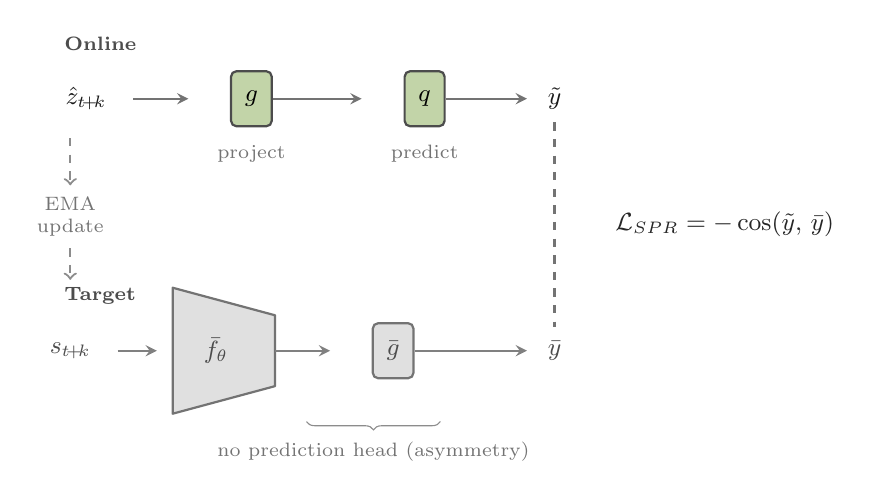
\begin{tikzpicture}[
    box/.style={draw=black!70, thick, minimum height=0.7cm,
                font=\small, inner sep=5pt, rounded corners=2pt},
    arr/.style={->, thick, >=stealth, black!55},
    lbl/.style={font=\scriptsize, text=black!55},
]

% === Online path (top) ===
\node[font=\scriptsize\bfseries, text=black!70, anchor=west] at (-0.7, 0.7) {Online};

% z_hat_{t+k} input
\node[font=\small, text=black!90] at (-0.3, 0) {$\hat{z}_{t\!+\!k}$};
\draw[arr] (0.3, 0) -- (1.0, 0);

% Projection
\node[box, fill=sprcomp] (proj) at (1.8, 0) {$g$};
\node[lbl] at (1.8, -0.7) {project};

\draw[arr] (proj.east) -- (3.2, 0);

% Prediction head
\node[box, fill=sprcomp] (pred) at (4.0, 0) {$q$};
\node[lbl] at (4.0, -0.7) {predict};

% Online output -- align at x=5.65 for clean vertical comparison
\draw[arr] (pred.east) -- (5.3, 0);
\node[font=\small, text=black!90] (ytilde) at (5.65, 0) {$\tilde{y}$};

% === Target path (bottom) ===
\node[font=\scriptsize\bfseries, text=black!70, anchor=west] at (-0.7, -2.5) {Target};

% s_{t+k}
\node[font=\small, text=black!70] at (-0.5, -3.2) {$s_{t\!+\!k}$};
\draw[arr, black!50] (0.1, -3.2) -- (0.6, -3.2);

% EMA Encoder (trapezoid)
\fill[targetfade, draw=black!55, thick, line join=round]
    (0.8, -4.0) -- (0.8, -2.4) -- (2.1, -2.75) -- (2.1, -3.65) -- cycle;
\node[font=\small, text=black!70] at (1.35, -3.2) {$\bar{f}_\theta$};

\draw[arr, black!50] (2.1, -3.2) -- (2.8, -3.2);

% EMA Projection
\node[box, fill=targetfade, draw=black!55, text=black!70]
    (tproj) at (3.6, -3.2) {$\bar{g}$};

% Target output -- align at x=5.65 to match online output
\draw[arr, black!50] (tproj.east) -- (5.3, -3.2);
\node[font=\small, text=black!70] (ybar) at (5.65, -3.2) {$\bar{y}$};

% === Cosine similarity ===
% Single vertical dashed line connecting y_tilde and y_bar
\draw[thick, dashed, black!55]
    (5.65, -0.3) -- (5.65, -2.9);
\node[font=\small, text=black!85, anchor=west] at (6.3, -1.6)
    {$\mathcal{L}_{\text{SPR}} = -\cos(\tilde{y},\, \bar{y})$};

% No prediction head annotation
\draw[decorate, decoration={brace, amplitude=3pt, mirror}, black!45]
    (2.5, -4.1) -- (4.2, -4.1)
    node[midway, below=4pt, font=\scriptsize, text=black!55]
    {no prediction head (asymmetry)};

% EMA update arrow (between the two paths)
\node[font=\scriptsize, text=black!55, align=center]
    at (-0.5, -1.5) {EMA\\update};
\draw[->, thick, dashed, black!45]
    (-0.5, -0.5) -- (-0.5, -1.1);
\draw[->, thick, dashed, black!45]
    (-0.5, -1.9) -- (-0.5, -2.3);

\end{tikzpicture}
\caption{Self-predictive loss. The predicted representation
  $\tilde{y}$ from the online path is compared to the target
  $\bar{y}$ from an EMA copy of the encoder via cosine similarity.
  The prediction head $q$ appears only on the online side, creating
  the asymmetry that prevents both paths from collapsing to a
  trivial constant.}
\label{fig:spr-loss}
\end{figure}
